% Model framework - similar to materials and methods, but with more paragraph
% continuity

\subsection*{Framework Conception and Configuration}

As mentioned before, the functionality of a protein strongly depends on its 3D structure, 
so that changes in its conformation (mutations) can affect how a protein interacts with its 
surroundings \cite{Sikosek2014Prot}. In this aspect, $A_G$ gives intrinsic information 
about complementarity between pairs of proteins and hence paths on the protein network are 
relevant for the prediction task. 

The proposed framework for prediction of protein-protein interactions consists of the
combination of the path counting metrics along with the vector representations of the
edges of the network (node2vec embeddings). Namely, the path counting metrics are either 
the counting of paths of length 2 (matrix $A_G^2$), the counting of paths of length 3 
(matrix $A_G^3$) or the degree-normalized counting of paths of length 3 (matrix $L_3$). 
The information retrieved from these matrices will be addressed from now on as A2, A3 
and L3, respectively.

Figure \ref{fig:framework} shows the proposed framework for predicting protein-protein interactions. As the 
framework combines two sources of information, it consists of three processes: (a) Metrics 
calculation and initial predictions, (b) Node and edge embeddings and (c) Machine Learning 
prediction.

\begin{figure}[h]
\caption{\label{fig:framework}Framework scheme}
	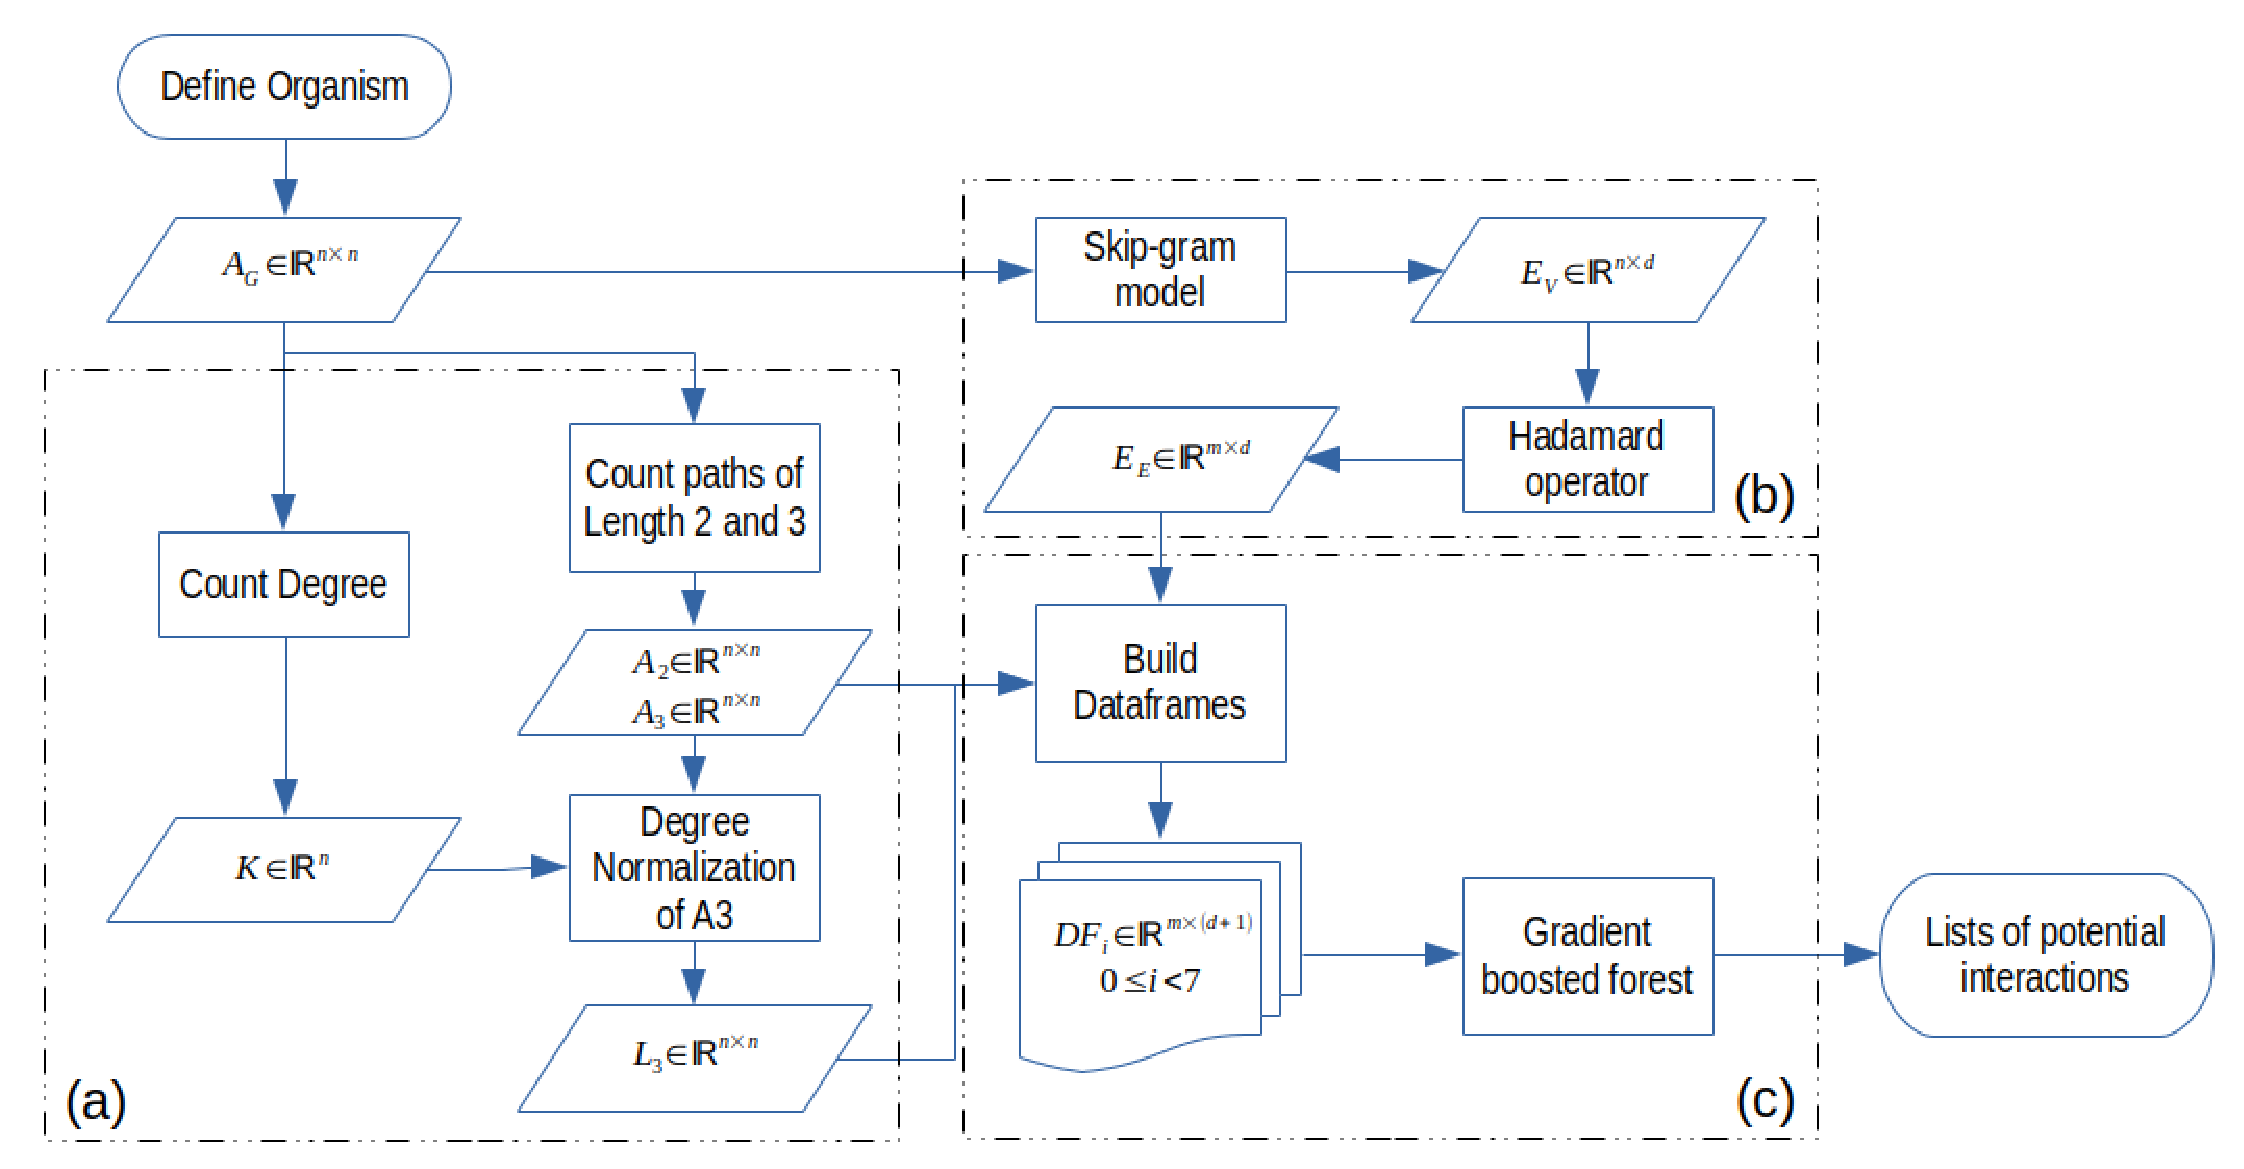
\includegraphics[width=\textwidth ]{figures/framework.eps}
\end{figure}

The input for the workflow consists of a representation of the connectivity of the network.
Online databases of protein-protein interactions usually report this information as an 
adjacency list with some additional attributes about the quality of this interaction. Namely, 
this data is represented as a list of pairs of identifiers and zero or more attributes for 
each pair. The framework only needs to know whether an interaction exists and therefore this 
additional information needs to be discarded in advance. In order to calculate optimally the
subsequent metrics, the framework creates the adjacency matrix $A_G$ out of the given list. 
Note that as no attributes from nodes or edges are added, the framework predicts based only 
on the intrinsic properties of the network related to connectivity. 

\subsubsection*{A. Metrics Calculation}
The goal of this stage is to build matrices $A2$, $A3$ and $L3$ which quantify, 
the number of paths of length 2, of length 3 and the degree-normalized count of 
paths of length 3, respectively. For this purpose, two calculations are done: 
counting the degree of each node ($k_i \in \mathbb{Z}$) and raising $A_G$ to the 
second to obtain $A2$. Finally, $A3$ and $L3$  are calculated simultaneously. 
Entries $L3_{i,j}$ of $L3$ can be calculated as 

\begin{equation}
  L3_{i,j}=\sum_{p,q\in V}\frac{{A_G}_{i,p}\cdot {A_G}_{p,q}\cdot {A_G}_{q,j}}{\sqrt{k_{p}\cdot k_{q}}}
\end{equation}

\subsubsection*{B. node2vec Embeddings}
The purpose of this step is to retrieve a vector representation of the network 
structure and thus be able to feed the Machine Learning model and improve its 
predictions. This is done using a state-of-the-art algorithm called node2vec, 
which is based on the word2vec technique to learn learn word associations from
a corpus of text. Instead of sentences, node2vec uses 
random walks from each node in order to construct a skip-gram model and a neural 
network to learn features (embeddings) from the nodes\cite{Grover_2016}. These 
features consist of a $d$-dimensional vector representation of each node.
Since the framework aims to predict edges, these node embeddings are used as 
input for the Hadamard operator to calculate edge embeddings. Namely, the edge 
embedding of edge $c_i,j$ is calculated as the element-wise product of each 
component of the node embeddings for nodes $i$ and $j$. $d$ is chosen as 16.

\subsubsection*{C. Machine Learning Prediction}
Finally, this stage aims at gathering information from the previous steps to 
enrich the prediction of a Machine Learning (ML) model and improve its results. 

The selected implementation for this prediction problem is XGBoost, which 
uses gradient boosted decision trees to learn whether an interaction is feasible. 
The first step in this process is to combine the two sources of information into 
Dataframes for each of the metrics: for each edge, the information from one of the 
metrics (A2, A3 or L3) is appended to the vector representation of $d$ dimensions 
from node2vec, resulting in 3 different tables. Dataframes including only one 
source of information (each metric or node2vec data) are also generated and 
fed to XGBoost for comparison.

For each metric, the initial prediction in step A is used to train the supervised 
ML model 


\subsection*{Framework Evaluation on the Human Interactome}

As the first step in the evaluation of A2, A3 and L3 metrics to assess link
prediction, the full calculation and ranking of all predictions was
carried out. The results for the analyzed human interactomes (\emph{HI-II-14}
and \emph{HI-TESTED}) is shown in Figure \ref{fig:HI1}, in which
the x axis represents a rank position $k$ and the y axis displays
the precision for the top $k$ predictions of each method, when assuming
interactome \emph{HI-III} as the validation set. 
	
\begin{figure}[h]
\caption{\label{fig:HI1}Methods Comparison for \emph{HI-II-14} and \emph{HI-TESTED}}
	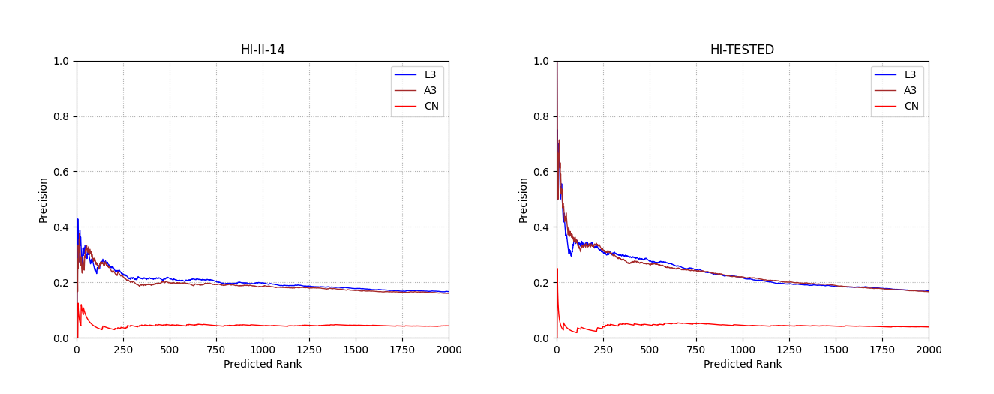
\includegraphics[width=\textwidth ]{figures/figure2.eps}
	%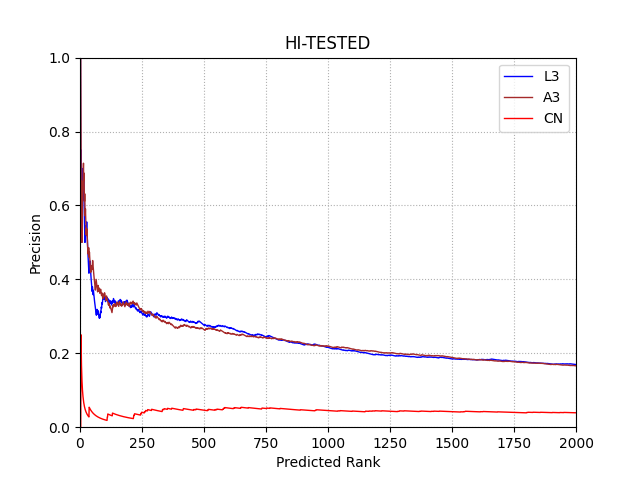
\includegraphics[width=0.7\textwidth ]{../hi-tested.txt.}
\end{figure}

As it can be inferred from the plots, L3-based predictions outperform
their $A{{}^2}$ counterparts. Results also show that L3-score and
$A^{3}$predictions follow a very similar trend.

However, the interest of this study is to assess if Machine Learning can boost
the overall performance on the prediction, so the proposed procedure
is adapted to the human interactome data: Instead of having to remove
a fraction of edges from the network in order to predict and validate,
the prediction network and the validation networks are given beforehand.
The rest of the procedure is carried out as mentioned above.
Table \ref{T1} presents the results for the combinations of Node2Vec
with each feature.

\begin{table}
\caption{\label{T1}Summary statistics for human interactomes}
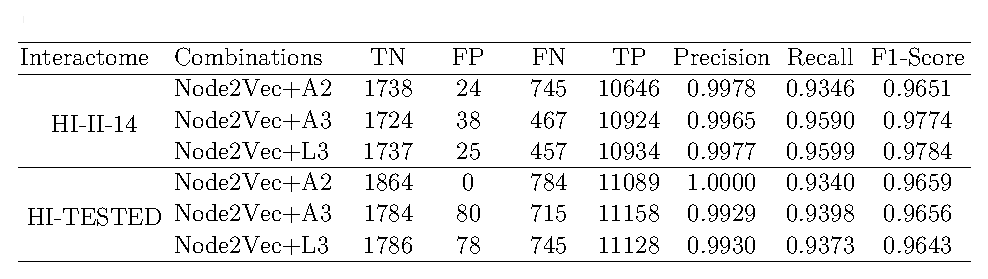
\includegraphics[width=1\columnwidth]{figures/T1}
\end{table}

In general, performance of all models is above 0.96 in terms of F1-Score.
Although marginally, the A2 feature-enriched model for HI-TESTED performs
better than their counterparts based on paths of length 3. The opposite
is also true for HI-II-14: models enriched with L3 and A3 features
perform better than their A2 counterpart. Results for the Interactome
\emph{HI-II-14} with Node2Vec and each metric are presented in Figures
S\ref{HI1}, S\ref{HI2} and S\ref{HI3}. It can be seen that for
\emph{HI-II-14}, A2 performs marginally better than L3 when comparing
precision but worse in terms of recall, although all metrics have
AUC values of 0.99.

On the other hand, the interactome \emph{HI-TESTED} was assessed with
the same methodology as \emph{HI-II-14} and results are shown in Figures
S\ref{HI1-1}, S\ref{HI2-1} and S\ref{HI3-1}. For this interactome,
A2 performs better in terms of false positives than A3 and L3, but
in terms of false negatives, A3 actually performs better that A2 and
L3. In terms of AUC, metrics results are indistinguishable. 

An interesting assessment from this human datasets can be observed
when looking at the importance plots, which show a very biased influence
of the handcrafted features. Figure \ref{F8-importance-H1} shows
this behavior for the \emph{HI-II-14} dataset, which is very similar
to \emph{HI-TESTED} (Figure S\ref{F8-importance-H2}).

\begin{figure}[h]
\noindent \begin{centering}
\caption{\label{F8-importance-H1}Importance gain plots for \emph{HI-II-14}}
\par\end{centering}
\begin{centering}
\includegraphics[width=0.48\columnwidth]{figures/Human/Imp\lyxdot A2\lyxdot 1\lyxdot eps}\includegraphics[width=0.48\columnwidth]{figures/Human/Imp\lyxdot A3\lyxdot 1\lyxdot eps}
\par\end{centering}
\centering{}\includegraphics[width=0.48\columnwidth]{figures/Human/Imp\lyxdot L3\lyxdot 1}
\end{figure}